%% Based on a TeXnicCenter-Template by Gyorgy SZEIDL.
%%%%%%%%%%%%%%%%%%%%%%%%%%%%%%%%%%%%%%%%%%%%%%%%%%%%%%%%%%%%%
%
%------------------------------------------------------------
%
\documentclass[a4paper,12pt,reqno]{article}
%----------------------------------------------------------
\usepackage{amsfonts}
\usepackage{graphicx}
\usepackage{geometry}
\usepackage{color}
\usepackage{amssymb,amsmath}
\usepackage{polski}
\usepackage[T1]{fontenc}
\usepackage[utf8]{inputenc}
\usepackage{caption}
\geometry{margin=1.1in}
\usepackage{wrapfig}
\usepackage{lipsum}  
\usepackage{listings}
\usepackage[toc,page]{appendix}
\usepackage{url}

\definecolor{codegreen}{rgb}{0.5, 0.09, 0.09}
\definecolor{codegray}{rgb}{0.5,0.5,0.5}
\definecolor{codepurple}{rgb}{0.58,0,0.82}
\definecolor{backcolour}{rgb}{0.94,0.94,0.94}
\definecolor{gray}{rgb}{0,0.6,0}

\lstdefinestyle{mystyle}{
    backgroundcolor=\color{backcolour},  
    commentstyle=\color{codegreen},
    keywordstyle=\color{blue},
    numberstyle=\tiny\color{codegray},
    stringstyle=\color{codepurple},
	basicstyle=\footnotesize\fontfamily{cmtt}\selectfont,
    breakatwhitespace=false,         
    breaklines=true,
    captionpos=b,
	language=C++,
    keepspaces=true,                 
    numbers=left,                    
    numbersep=5pt,                  
    showspaces=false,                
    showstringspaces=false,
    showtabs=false,                  
    tabsize=2
}
 
\lstset{style=mystyle}
\lstset{literate=%
    *{0}{{{\color{gray}0}}}1
    {1}{{{\color{gray}1}}}1
    {2}{{{\color{gray}2}}}1
    {3}{{{\color{gray}3}}}1
    {4}{{{\color{gray}4}}}1
    {5}{{{\color{gray}5}}}1
    {6}{{{\color{gray}6}}}1
    {7}{{{\color{gray}7}}}1
    {8}{{{\color{gray}8}}}1
    {9}{{{\color{gray}9}}}1
}
%------------------------------------------------------------
\begin{document}

%\begin{figure}[h]
%	\centering
%		\includegraphics[width=0.40\textwidth]{logo.pdf}
%\end{figure}


\begin{center}

\thispagestyle{empty}

%UNIWERSYTET WROCŁAWSKI\\
\Large 
Uniwersytet Wrocławski\\
Wydział Fizyki i Astronomii\\
\vspace{0.8cm}
\vspace{1.8cm}

\Large Krzysztof Kukiz \\
\vspace{3.2cm}
\Large \textbf{INTELIGENTNE POWITANIE} \\
\vspace{1.5cm}
INTELLIGENT GREETING
\end{center}
\vspace{3.7cm}
\begin{flushright}
\large{ Praca inżynierska na kierunku \\Informatyka Stosowana i Systemy Pomiarowe \\}
\vspace{0.5cm}
\large{ Opiekun \\ dr hab. Maciej Matyka, prof. UWr}
\end{flushright}
\vspace{2.2cm}

\begin{center}
\large Wrocław, \today
\end{center}

\newpage

\tableofcontents

\newpage

%
%	Streszczenie PL
%
\begin{flushleft}
\Large \textbf{Streszczenie}
\end{flushleft}
\vspace{1cm}
Niniejsza praca przedstawia projekt systemu inteligentnego rozpoznawania osób oraz podejmowania przez system wcześniej zdefiniowanych działań, w zależności od rozpoznanej osoby. W przypadku braku rozpoznania osoby, system poda także odpowiedni komunikat głosowy oraz wizualny. 
\newline
Projekt oparty jest na Raspberry Pi 4B, na języku programowania python 3\textcolor{red}{, oraz} wykorzystuje elementy wydrukowane na drukarce 3D Creality Ender-3 v.2
\newline
Projekt łączy ze sobą w całość 3 warstwy niezbędne do wykonania wszystkich założonych zadań w taki sposób aby w przyszłości można było rozbudować system o kolejne funkcjonalności.
\begin{enumerate} % itemize
  \item Warstwę sprzętową składającą się z czterech \textcolor{red}{głównych} elementów.
  \begin{itemize}
  	\item kamery, stanowiącej element wejściowy sygnału i odpowiedzialnej za pobranie sygnału video z otoczenia
  	\item micro-komputera Rasppery Pi, odpowiedzialnej za przetworzenie sygnału oraz z kamerki, oraz sprawdzenie czy zdjęcie danej osoby znajduje się w bazie danych oraz wypowiedzenia odpowidniego komunikatu
  	\item głośnika, stanowiącego element wyjściowy z systemu i służącego do podawania komunikatów głosowych. Głośnij jest podpinany pod port jack 3,5mm, zatem istnieje możliwość zastosowania dowolnego głośnika.
  	\item Wyświetlacza, na którym generowana jest część wizualną powitania. Wyświetlacz jet podłączony do Raspberry Pi
  \end{itemize}
  \item Warstwę programistyczną odpowiedzialną za:
  \begin{itemize}
  	\item obróbkę oraz optymalizację odczytanego obrazu
  	\item interpretację pobranego obrazu oraz porównanie go z wcześniej zdefiniowaną bazą zdjęć
  	\item podjęcie decyzji o tym jakie działanie ma być podjęte oraz wygenerowanie właściwego sygnału skutkującego podjęciem określonych działań
  \end{itemize}
  \item Warstwę produktową w postaci dedykowanej, zaprojektowanej specjalnie dla tego projektu obudowy, pełniącej 3 podstawowe funkcje:
  \begin{itemize}
  	\item Organizacyjną, zapewniającą spójną organizację podzespołów oraz ich prawidłową wentylację pasywną
  	\item Ochronną, zabezpieczającą podzespoły użyte w projekcie przed uszkodzeniem
  	\item Informacyjną, zawierającą podstawowe informacje o produkcie
  \end{itemize}
\end{enumerate}
Celem projektu było stworzenie systemu mobilnego, o jak najmniejszych wymiarach, który jest gotowy do działania natychmiast po podłączeniu zasilania.

%
%	Streszczenie EN
%
\newpage
\begin{flushleft}
\Large \textbf{Abstract}
\end{flushleft}
\vspace{1cm}
This work presents the design of a system for the intelligent recognition of persons and for the system to take predefined actions, depending on the recognised person. If the person is not recognised, the system will also give an appropriate voice and visual message.
\newline
The project is based on a Raspberry Pi 4B, the python 3 programming language, and uses components printed on a Creality Ender-3 v.2 3D printer
\newline
The project brings together the 3 layers needed to carry out all the tasks in such a way that the system can be extended in the future with further functionalities.
\begin{enumerate} % itemize
  \item A hardware layer consisting of four main components.
  \begin{itemize}
  	\item the camera, which is the signal input element and is responsible for collecting the video signal from the environment
  	\item the Rasppery Pi microcomputer, which is in charge of processing the signal from the camera, checking whether a given person's photo is in the database and issuing an appropriate message
  	\item A speaker that is an output from the system and is used to give voice announcements. The speaker plugs into a 3.5mm jack port, so any speaker can be used.
  	\item A display on which the visual part of the greeting is generated. The display is connected to the Raspberry Pi
  \end{itemize}
  \item The programming layer responsible for:
  \begin{itemize}
  	\item processing and optimisation of the read image
  	\item interpretation of the retrieved image and comparison with a predefined image database (library)
  	\item deciding on the action to be taken and generating the right signal to take the specified action
  \end{itemize}
  \item A product layer in the form of a dedicated enclosure \textcolor{red}{(Etui)}, designed specifically for this project, performing 3 basic functions:
  \begin{itemize}
  	\item Organisational, to ensure consistent organisation of the components and their proper passive ventilation
  	\item Protective, to prevent damage to the components used in the project
  	\item Information, including basic product information
  \end{itemize}
\end{enumerate}
The aim of the project was to create a mobile system with the smallest possible dimensions, which is ready for operation as soon as the power is connected.


\newpage

%
%	Wstęp
%
\section{Wstęp}
\subsection{Wprowadzenie}
Systemy inteligentne są stosowane obecnie na całym świecie. Znajdują coraz szersze zastosowanie w życiu codziennym każdego z nas zarówno w pracy jak i w domu. Potrafią reagować na nasze zachowania, odczytywać intencje oraz gromadzić i wykorzystywać dane, które im udostępnimy zarówno na poziomie jednostki, jak i całych grup społecznych.
\newline
W naszym codziennym życiu są elementem składowym inteligentnych budynków opartych między innymi o systemy LOXONE, KNX, AMPIO, czy też FIBARO i znacznie ułatwiają codzienne czynności poprzez sterowanie klimatem, ogrzewaniem, rekuperacją, czy też podlewaniem ogrodów, sprzątaniem, a nawet optymalnym wykorzystaniem energii elektrycznej.
\newline
Systemy inteligentne pomimo swoich kosztów zdobywają coraz większą popularność nie tylko w zastosowaniach profesjonalnych, ale także w zastosowaniach prywatnych i mogą być oparte zarówno o infrastrukturę przewodową (patrz rys. (\ref{kable})), jak i mogą być oparte na rozwiązaniach bezprzewodowych.
\begin{figure}[!ht]%
\centering
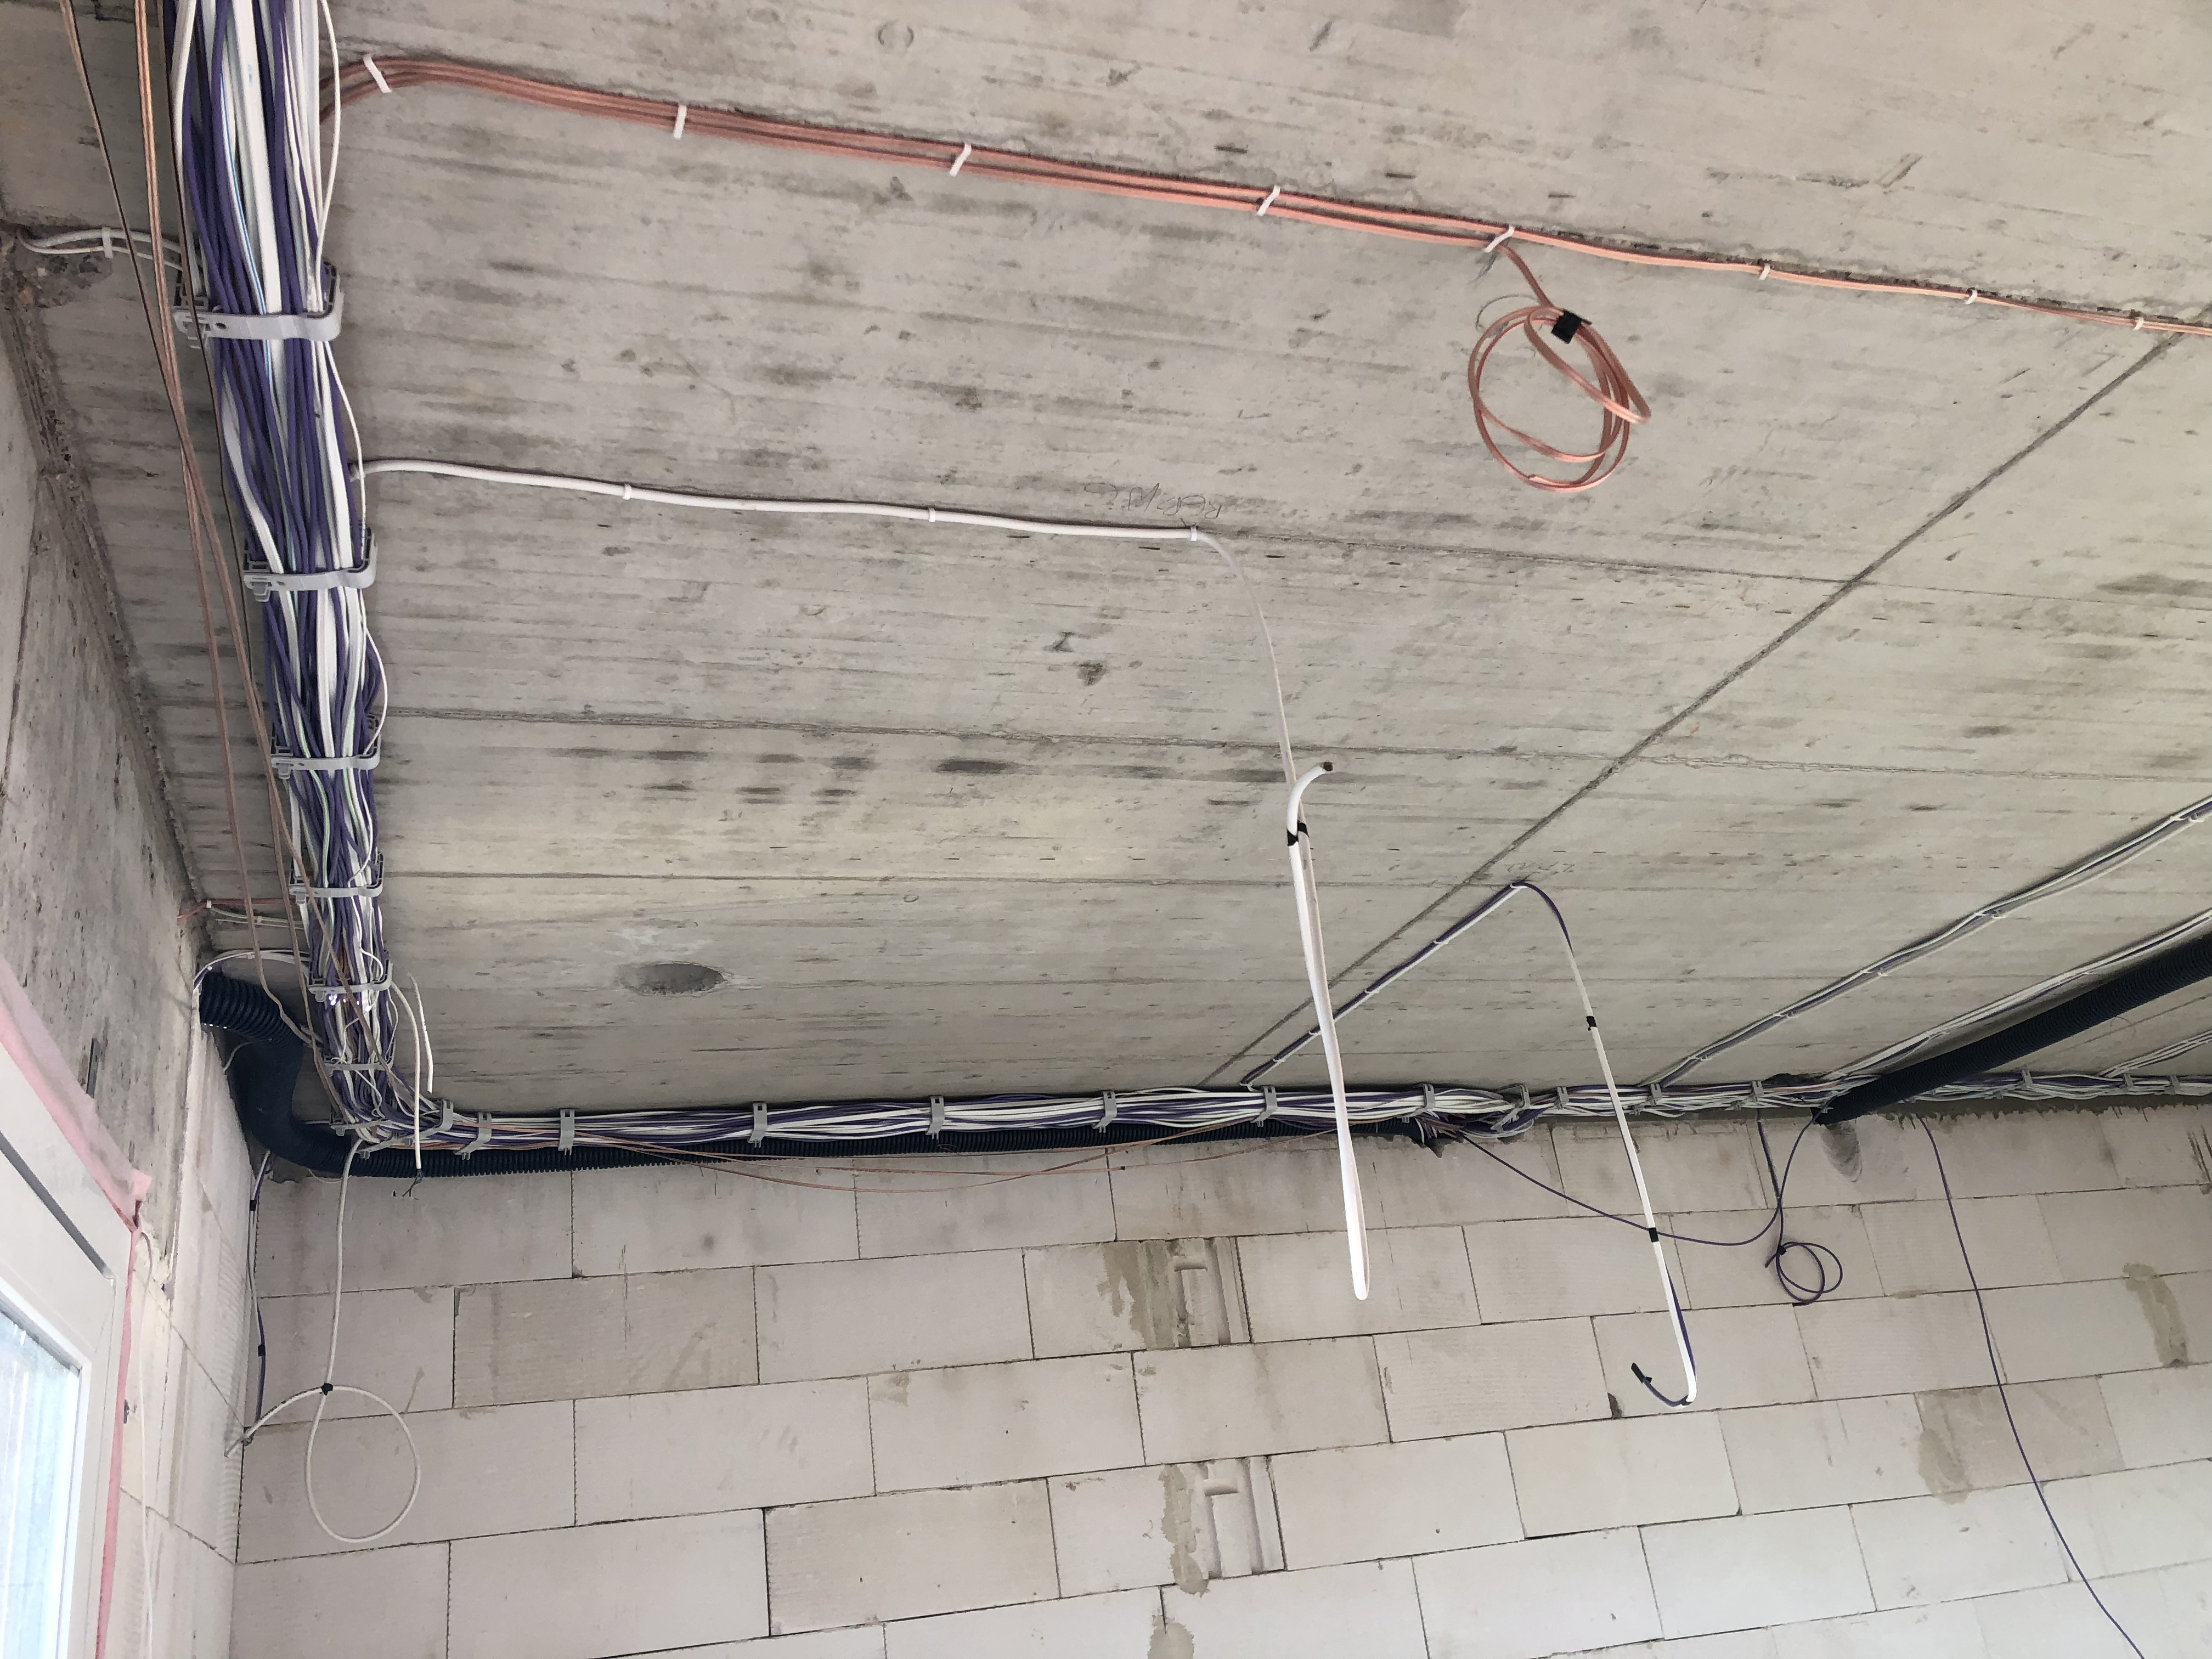
\includegraphics[width=0.8\columnwidth]{imgs/domkable.png}
\caption{Przykład okablowaniem domu inteligentnego. [źródło: materiały własne] \label{kable}}
\quad
\end{figure}
\newline
Żaden system nie posiada jednak wszystkich funkcjonalności, które są niezbędne danemu użytkownikowi. W większości z nich brakuje mobilnego systemu pozwalającego na rozpoznanie osób oraz podjęcia konkretnych działań w zależności od osoby, która została zidentyfikowana.
\newline
System inteligentnego rozpoznawania osób, który jest tematem niniejszego projektu, pozwala właśnie na identyfikację osób wchodzących do pomieszczenia na podstawie zapisanej wcześniej bazy zdjęć oraz powitanie ich indywidualnym komunikatem zarówno głosowym, jak i wizualnym.
\newline
Do realizacji projektu wykorzystałem \textcolor{red}{micro-komputer} Raspperry Pi 4B oraz język programowania Python 3. Jako elementu wejściowego sygnału użyłem kamery Raspberry Pi Camera HD v2 8MPx zgodnej z Raspperry Pi 4B, oraz najzwyklejszego głośnika pod wejscie jack 3,5mm
\subsection{Cel i zakres pracy}
Celem głównym projektu jest stworzenie prototypu inteligentnego, mobilnego systemu rozpoznawania osób, na podstawie wcześniej zgromadzonej bazy zdjęciowej, a także wygenerowanie unikatowego powitania głosowego oraz wizualnego w zależności od rozpoznanej osoby.
\newline
Celami szczegółowymi projektu są wybór technologii sprzętowej, wybór technologii programistycznej oraz zaprojektowanie i wykonanie obudowy prototypu, mieszczącej wszystkie elementy projektu
\newline
Praca swoim zakresem obejmuje zarówno tematykę z dziedziny elektroniki, informatyki projektowania oraz prototypowania 3D.
\newline
W zakresie elektroniki wykorzystane zostały układy i sensory zgodne z płytką Rasppery 4B, w zakresie informatyki napisany został program w języku Python 3 i wykorzystujący do realizacji zadań dostępne biblioteki, natomiast w zakresie prototypowania z wykorzystaniem druku 3D, użyta została drukarka 3D Creality Ender v2 oraz materiał \textcolor{red}{PET-G}. Do celów zaprojektowania obudowy wykorzystano program SOLIDWORKS.
\newline
Projekt z jednej strony pokazuje, że połączenie wiedzy z zakresu elektroniki, informatyki oraz projektowania dostarcza każdemu studentowi odpowiednią wiedzę oraz umiejętności, do wykonania prototypu od fazy projektowej do fazy praktycznego zastosowania,  z drugiej udowadnia, że wiedza ta pozwala na wykonania projektu z wykorzystaniem elementów ogólnodostępnych na rynku.
\subsection{Struktura pracy} % tutorial jak prrace czytać

\newpage
\section{Wymagania stawiane projektowi}

\newpage
\section{Oczekiwane funkcjonalności projektu}

\newpage
\section{Warstwa sprzętowa}
\subsection{Kamera jako element wejściowy}
\subsection{Płyta Raspberry Pi}
\subsection{Głośnik jako element wyjściowy}
\subsection{Ekran jako element wyjściowy}

\newpage
\section{Warstwa programistyczna}
\subsection{Python jako język programowania}
\subsection{Biblioteki}
\subsection{Algorytm}
\subsection{Kod}

\newpage
\section{Warstwa produktowa}
\subsection{Technologia druku 3D}
\subsection{Projekt obudowy}
\subsection{Wykonanie obudowy}

\newpage
\section{Realizacja projektu}
\subsection{Napotkane problemy}
\subsection{Możliwości rozbudowy}

\newpage
\section{Wnioski}

\newpage

\bibliographystyle{plain}
\bibliography{praca_dyplomowa_krzysztof_kukiz}


\newpage

\begin{equation} 
\rho\left(\frac{\partial\vec v}{\partial t}+(\vec v\cdot\nabla)\vec v\right) =\rho\vec f - \nabla p + \mu\triangle\vec v, \label{rownanie}
\end{equation} 

\begin{figure}[!ht]%
\centering
\includegraphics[scale=0.85]{logo.eps}
\caption{Podpis rysunku, który jest obrazem wektorowym (EPS). \label{logotyp}}
\qquad
\end{figure}   

\begin{figure}[!ht]%
\centering
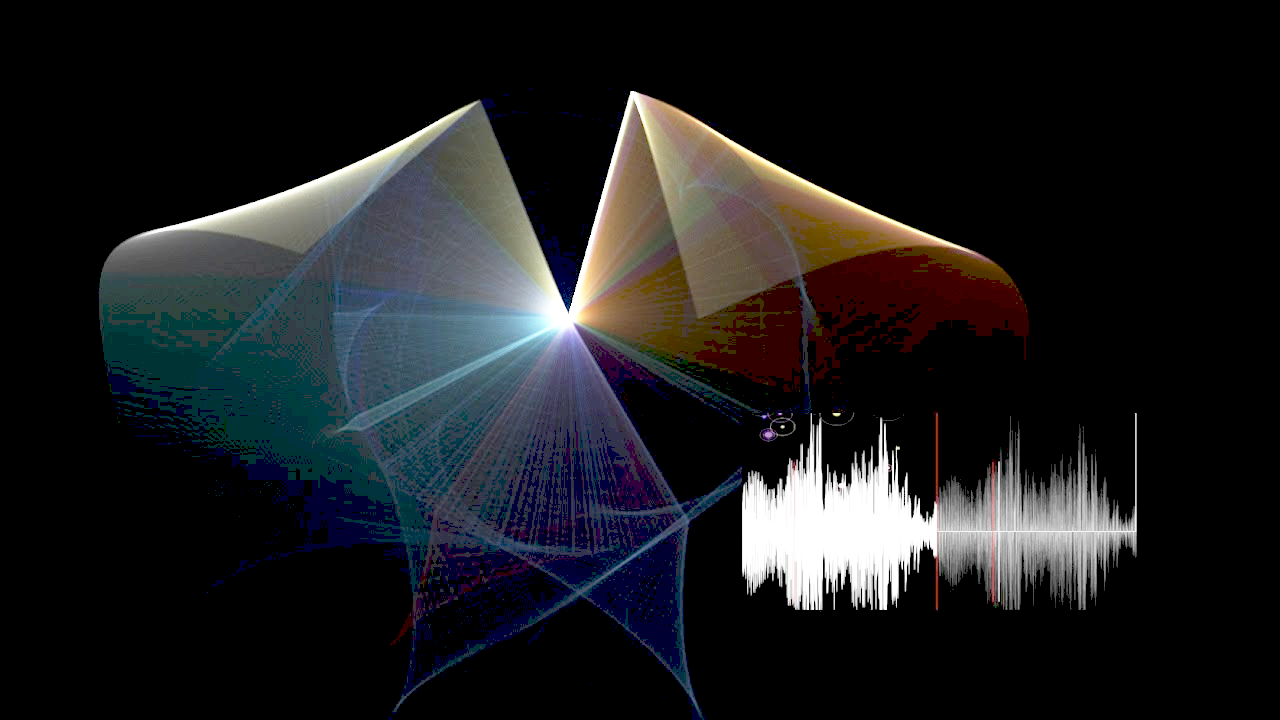
\includegraphics[width=0.8\columnwidth]{pendulums.png}
\caption{To jest rysunek drugi, kilkadziesiąt wahadeł podwójnych z syntezą dźwięku.\label{wahadla}}%
%
\qquad
\end{figure} 

\end{document}




